\subsection{STM32F1xx /\cm{1}/} \label{stm32f1}

\subsubsection{Демо-плата STM32VLDISCOVERY /MB913C/}

Отладочный комплект для линейки МК STM32F100 Value 
Line\ --- с контроллером STM32F100RB(T6B).

\begin{wrapfigure}{r}{0.25\textwidth}
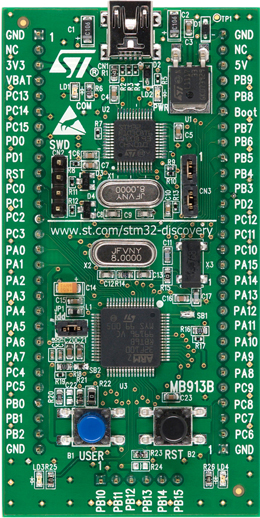
\includegraphics[height=0.7\textheight]{fig/STM32VLDISCOVERY.jpg}
\end{wrapfigure}

\url{www.st.com/stm32-discovery}
\bigskip

\vld\ --- дешевый и быстрый способ освоение линейки МК STM32 
value line. 
Плата содержит необходимый минимум для начинающих и опытных пользователей
для быстрого старта.
\vld\ включает МК STM32F100RB в корпусе LQFP64, внутрисхемный 
отладчик/программатор ST-Link (обрезанный v.1) для отладки прошивок.
В комплекте предоставляется большое количество готовых примеров прошивок
в исходных текстах, для обеспечения быстрого запуска и изучения, с примерами
использования светодиодов, кнопок и доступа к контактным гребенкам
для подключения к другим платам или устройствам.

\bigskip
\begin{itemize}
\item МК STM32F100RB, 128 KB Flash, 8 KB RAM в корпусе LQFP64
\item Наплатный ST-Link с джамперами для переключения в режим независимого 
программатора (с интерфейсом SWD)
\item Питание от USB или внешнего источника 5 V или 3.3 V
\item Может обеспечить питанием целевую схему 5 V или 3 V
\item Два светодиода (зеленый и синий)
\item Одна пользовательская кнопка, вторая --- сброс
\item Контактные гребенки для всех выводов QFP64 для быстрого подключения
при прототипировании и подключения логического анализатора
\end{itemize}
